\documentclass[../../Problems]{subfiles}
\begin{document}
\subsection{Spiral Grid}
\textbf{Problem Statement:}\\
Generate a grid containing numbers from $1$ to $n^2$ such that $1$ is at center and then the numbers spiral outwards from $1$ in counterclockwise direction. Also, make sure each element of grid is equally spaced as shown in \ref{fig:spiralgrid}.
\begin{note}
	If $n$ is even then choose the left-bottom element from the four possible centers.
\end{note}
\begin{comment}
	\begin{figure}[H]
		\centering
		\begin{subfigure}{0.4\linewidth}
			\centering
			\begin{tabular}{rrrr}
			16 & 15 & 14 & 13 \\
			5  & 4  & 3  & 12 \\
			6  & 1  & 2  & 11 \\
			7  & 8  & 9  & 10
			\end{tabular}
			\caption{$n=4$}
		\end{subfigure}
		\begin{subfigure}{0.4\linewidth}
			\centering
			\begin{tabular}{rrrrr}
			17 & 16 & 15 & 14 & 13 \\
			18 & 5  & 4  & 3  & 12 \\
			19 & 6  & 1  & 2  & 11 \\
			20 & 7  & 8  & 9  & 10 \\
			21 & 22 & 23 & 24 & 25
			\end{tabular}
			\caption{$n=5$}
		\end{subfigure}
		\caption{Spiral Grid}
		\label{fig:spiralgrid}
	\end{figure}
\end{comment}
\begin{testcasesMore}
	{$t$ \hfill(number of test cases, an integer)\\$n_1\ n_2\ \ldots\ n_t$ \hfill($t$ space seperated integers for each testcase)}
	{Required spiral grid of $n_i^2$ numbers with appropriate spacing}
	{$1 \leq n_i \leq 100$}
	{5\\1 2 3 6 15}
	{\vspace{-2em}\begin{figure}[H]
		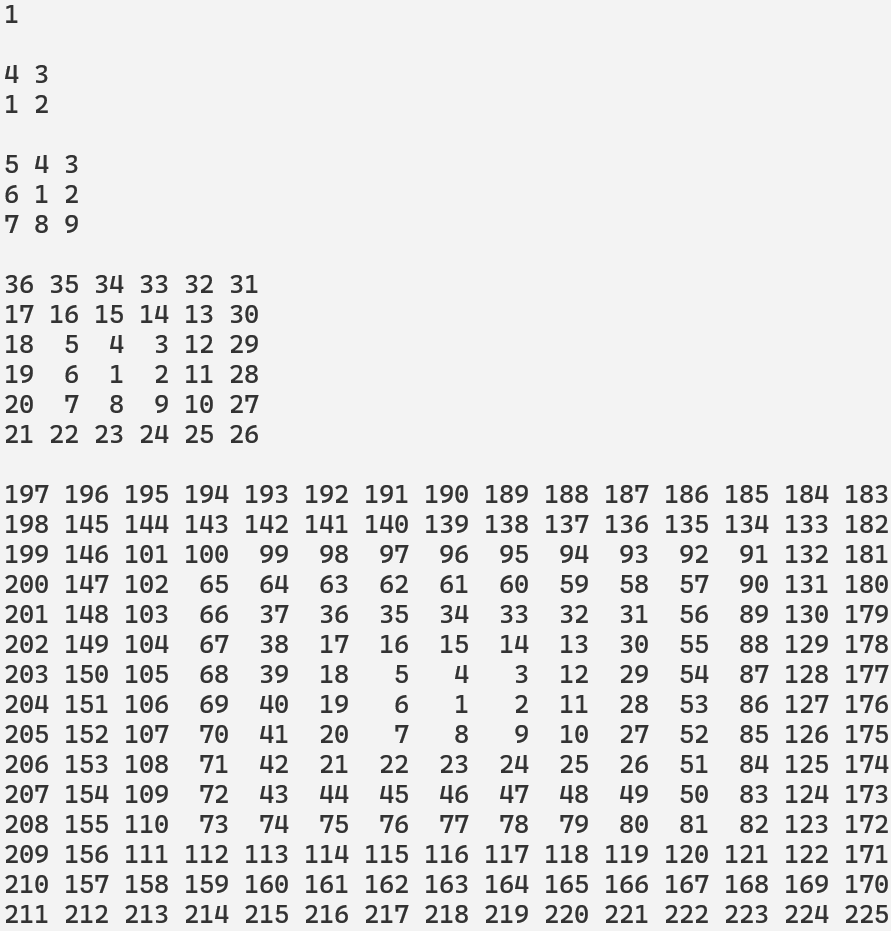
\includegraphics[width=0.5\linewidth]{Spiral Grid.png}
		\caption{Sample Output}
		\label{fig:spiralgrid}
	\end{figure}
	}
	{https://github.com/paramrathour/CS-101/tree/main/Test Cases/Spiral Grid/Input.txt}
	{https://github.com/paramrathour/CS-101/tree/main/Test Cases/Spiral Grid/Output.txt}
	{https://github.com/paramrathour/CS-101/tree/main/Starter Codes/Spiral Grid.cpp}
\end{testcasesMore}
\begin{funvideo}
\href{https://youtu.be/iFuR97YcSLM}{Prime Spirals -- Numberphile}
\end{funvideo}
\end{document}